\section{A reference design for a clause-governed safeguard}
\label{sec:design}

The evidence suggests a plausible role for typed decision models in a safeguard such as the \pol{} safety valve: a fast, cheap, recorded \emph{detector}, not a \emph{judge}.
\Cref{fig:architecture} sketches a design built on that principle for the valve of \clause{5.4.1}; it applies to any governance layer that screens the inputs and outputs of AI systems.
It is compatible with the pilot protocol of the NaturalDAO governance workstream, to which the author contributes and which already distinguishes \texttt{conforming}, \texttt{violating} and \texttt{insufficient} verdicts and the actions allow, repair, block, clarify and review~\cite{polgov}; the design adds a temporary \emph{hold} and makes \emph{block} final only after human confirmation.
Where a recommendation coincides with a choice already made in that protocol we say so, so that readers can judge whether the evidence or the prior design drove it.

\begin{figure}[t]
\centering
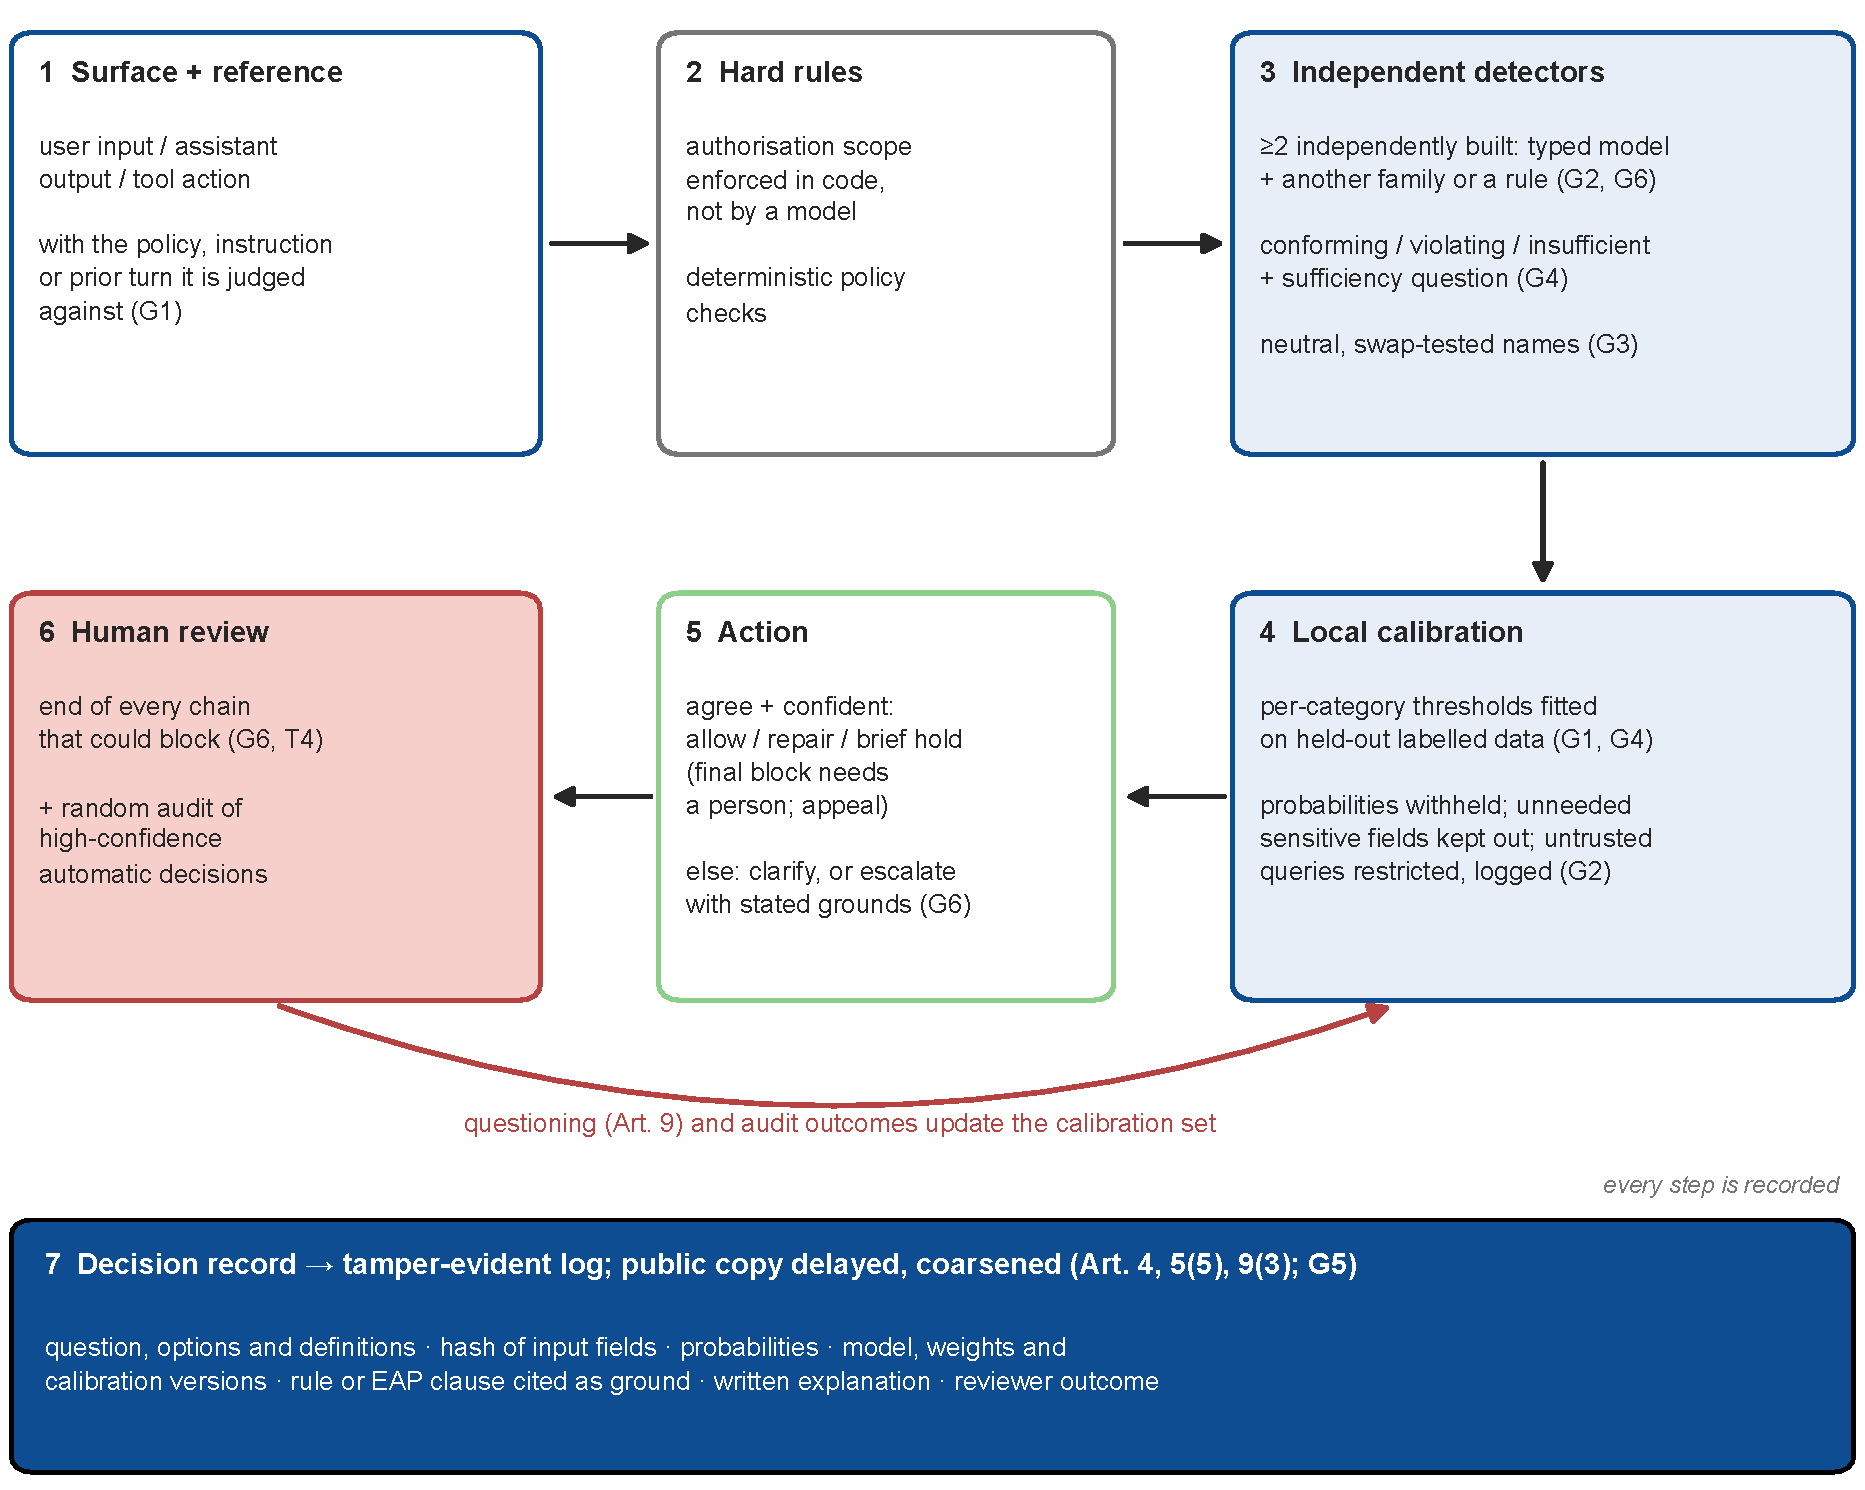
\includegraphics[width=0.8\linewidth]{figures/fig_architecture.pdf}
\caption{A reference design for a clause-governed safety valve. Typed models are detectors (3) whose output is calibrated locally (4) before any automatic action (5); disagreements and insufficient information are clarified or escalated, any final block is confirmed by a person, and a random sample of confident automatic decisions is audited by people (6); every step is written to a decision record (7). Labels in parentheses give the requirement or tension that motivates each element.}
\label{fig:architecture}
\end{figure}

The design has seven elements.
\begin{enumerate}
  \item \textbf{Give the detector the reference, not only the text.} Many failures are defined against an instruction, a policy or a prior statement~\cite{arx29429}; the content under review is always paired with that context. Facts that require computation or inference (sums, dates, consequences) are computed in code or in a separate logged step and written into the state, not left to the detector~\cite{arx39496,arx01834}.
  \item \textbf{Enforce scope in code.} Whether an agent stays within its authorisation is a property of the surrounding system~\cite{arx22664}, enforced by capability checks before any model is consulted.
  \item \textbf{Use at least two independently built detectors.} A blocking signal requires agreement between detectors that differ in construction, such as models of different families or a model and a rule, since peer models share confident errors~\cite{arx29769}, while agreement with a differently built rule let a reviewer skip about a third of cases without loss of macro-F1, although fewer disguised attacks were flagged as non-benign~\cite{arx02048}. Every question is three-valued (conforming, violating, insufficient), sufficiency is also asked as its own yes/no question~\cite{arx01006}, and options carry neutral identifiers bound to definitions and pass a renaming test~\cite{arx26758,arx00346}. Flags that must fail independently (allow/block, risk level, needs-human) are asked in separate calls, because in an open \jev{}-compatible model one planted note changed several answers in the same call~\cite{zen23038928}\zmark{}. Self-hostable models are preferred where their accuracy suffices (T3). The three-valued verdict is already part of the workstream's pilot protocol.
  \item \textbf{Calibrate locally, keep probabilities from untrusted callers and restrict what they can query.} Thresholds are fitted per category on held-out local data~\cite{arx29429,arx24052,jkf87_2026replication}, with distribution-free risk control where its exchangeability assumption is plausible~\cite{bates2021distribution,angelopoulos2024conformal}, and re-certified for every new question type~\cite{arx33689}, on a schedule, and whenever a temporal re-validation fails (item~16 of \cref{tab:checklist}). Raw probabilities are not returned to untrusted callers, because they help attackers optimise, although attacks also succeed with labels alone~\cite{arx30243,arx28613}; fields a decision does not need, sensitive attributes above all, are kept out of the detector's input, since a user authorised for the task, by planting conditional instructions in the input, recovered hidden attributes from labels alone with two to six queries per state; and queries from untrusted callers are restricted to authorised tasks, since labels refined harmful plans, and logged, since labels also trained a surrogate~\cite{arx04985}.
  \item \textbf{Act automatically only on agreement, and restrict people only briefly and reversibly.} Agreement plus calibrated confidence allows automatic \emph{allow}, automatic \emph{repair} of the AI system's own output (such as the truncation of \clause{4.3.3.1}, never the editing of a person's message), and a \emph{hold} of a person's content limited in time (for example, at most 24 hours) and fully reversible. A hold becomes a final block of a person's speech, a benefit or an account only after confirmation by a person, and remains open to appeal. Disagreement or \texttt{insufficient} leads to clarification or to escalation to a stronger reasoning model that must state its grounds~\cite{arx26550}. Because an automatic allow is consequential for anyone the allowed content harms, the miss rate is monitored and governed alongside the false-block rate. This element is what keeps the typed model a detector in the sense of \cref{sec:intro}.
  \item \textbf{End every chain that could block with a person, and audit confident decisions.} Reviewers see every escalation that would end in a block, every unresolved escalation and a random sample of high-confidence automatic decisions, since the most damaging errors are confident and shared~\cite{arx29769,arx33401}; their outcomes, and the results of public questioning under \art{9}, feed back into the calibration set.
  \item \textbf{Record every decision.} Each record holds the question, option set and definitions, a hash of the input fields, the probabilities, the model, weight and calibration versions, the rule or clause cited as ground, any written explanation, and the reviewer's outcome. Records are kept in a tamper-evident log open to supervisors (\art{9}(3)); the public version publishes probabilities coarsened and with a delay, so that it serves \art{4} and \art{5}(5) without becoming an oracle for attackers.
\end{enumerate}

\paragraph{Making human review workable.}
A person at the end of the chain is a safeguard only if the person can do the job.
Reviewers need capacity: strict error limits shift volume into review and blocking~\cite{arx33401}, and inserted opinions push confident answers into review~\cite{arx31142}, so review load must be budgeted and reported alongside accuracy, and cheaper evaluation may increase rather than reduce the total~\cite{arx01231}.
Reviewers are prone to automation bias and complacency~\cite{parasuraman2010complacency,green2022flaws} and can become the place where responsibility for system failures lands~\cite{elish2019moral}, so the model's verdict and probability are hidden during the random audit, and agreement between reviewers, not only with the model, is measured.
People also disagree on exactly the contested items where typed models are most over-confident~\cite{pavlick2019inherent,davani2022dealing,zen23032384}\zmark{}, so contested categories need more than one reviewer, and the person affected needs notice, reasons and a route of appeal~\cite{santaclara2021,dsa2022}.

\paragraph{Trade-offs and known limits of this design.}
Requiring two detectors to agree before blocking lowers sensitivity: more violations are missed, which conflicts with strict miss limits that are otherwise met by blocking more~\cite{arx33401}; the design accepts more holds and more review instead, and its miss rate must be measured.
Risk-control guarantees hold under exchangeability between calibration and deployment data; they bound error under benign drift, not under adaptive attack, which the G2 evidence shows is realistic.
For hate speech the shift is not hypothetical: across 20 language models, rankings on four static English hate-speech benchmarks did not predict rankings on time-stamped or neologism-substituted data (Spearman's $\rho$ between $-0.31$ and $0.19$, all 90\% intervals including zero), whereas the static benchmarks agreed with each other (mean $\rho = 0.36$)~\cite{dibonaventura2025hatevolution}.
Separate calls for independent flags and a second detector multiply cost and latency, eroding the main advantage of typed models, although the measured costs leave a wide margin~\cite{arx00346,arx01079}.
Finally, most elements rest on evidence of low or very low certainty (\cref{tab:keyfindings}); the design is a hypothesis to be tested on the \pol{} construct, not a validated system.

\Cref{tab:checklist} turns the evidence into a checklist for any typed model proposed for such a safeguard.
Items 1--4, 9, 14 and 15 draw on 9 of the 14 items of~\cite{arx32160} (its B1--B2, C1, C3--C4, R1--R2 and T2--T3); the others are added for a governance safeguard, and that checklist's B3, T1, T4, R3 and C2 are not adopted. Each item has a provisional pass criterion; the values are starting points to be set by those deploying the safeguard, not empirically validated thresholds.

\begin{table}[!htbp]
\centering
\footnotesize
\caption{Evaluation checklist with provisional pass criteria for a typed decision model in a governance safeguard. ``Basis'' gives the evidence or clause; items marked $\circ$ are added beyond the checklist of~\protect\cite{arx32160}.}
\label{tab:checklist}
\begin{tabularx}{\linewidth}{@{}rL>{\raggedright\arraybackslash}p{0.27\linewidth}>{\raggedright\arraybackslash}p{0.17\linewidth}@{}}
\toprule
\# & Requirement & Provisional pass criterion & Basis \\
\midrule
1 & Compare with a label-probability readout of a generative model and a cheap generative cascade & Reported on the same items & \cite{arx32160} \\
2 & Fit thresholds on held-out local data; report F1 at the fitted and the default threshold & Fitted threshold certified with a one-sided risk bound & \cite{arx29429,arx00346} \\
3 & Report calibration per category, before and after local recalibration & Per-category ECE and slope reported with intervals & \cite{arx24052,arx27607} \\
4 & Option-name swap test & Flip rate under a definition swap at most twice the repeat-noise floor & \cite{arx26758,arx00346} \\
5$^\circ$ & Three options including \texttt{insufficient}, plus a separate sufficiency question & Recall of \texttt{insufficient} at least 0.5 on paired present/absent items & \cite{arx39496,arx01006,polgov} \\
6$^\circ$ & Coherence of complementary and exclusive questions & Deviation from summing to one within twice repeat noise & \cite{arx33209} \\
7$^\circ$ & Red-team with adaptive, probability-guided additions, inserted opinions, lures and multi-turn attacks, and with label-only oracle attacks (attribute inference, surrogate extraction) under the deployed input and query restrictions & Attack success reported per attack type and below a target set in advance & \cite{arx30243,arx31142,arx01834,checkpoint2026jev,arx04985} \\
8$^\circ$ & Errors disaggregated by sub-type, including confident errors & No sub-type with recall below a set floor & \cite{arx33401} \\
9 & Decision-level stability over repeats, interfaces and decompositions & Disagreement across interfaces reported; one interface fixed per question & \cite{arx27678,arx37470,arx33971} \\
10$^\circ$ & Error correlation with every escalation target & Repetition of confident errors below independence plus a set margin & \cite{arx29769} \\
11$^\circ$ & Evaluation in Chinese and each language served, with script and order variants & Each language within a set margin of English & \cite{qin2026zhdecisionbench,typesafe_models} \\
12$^\circ$ & No forced choices between groups of people; group-bias test on behavioural questions & Error rates by group within a set margin & \cite{simmons2026saidno,sap2019risk} \\
13$^\circ$ & Value-laden questions: default position without persona, behaviour where people disagree & Reported; contested items routed to people & \cite{arx36399,zen23032384} \\
14 & Latency with and without caching; cost per correct decision & Reported, including review load & \cite{arx32160,arx00346} \\
15 & Versions and inspectability & Model, weights and calibration versions pinned in each record; self-hostable or logged & \art{4}, \art{5}(4)--(5), \clause{5.5} \\
16$^\circ$ & Temporal re-validation: re-evaluate on a time-stamped hold-out of recent items and on paired items in which a target word is replaced by a newly emerged term of the same meaning & In each language served (item 11): per-period recall of hate language within a set margin of the certification period, and flip rate on neologism pairs within a set margin of the repeat-noise floor; when either is exceeded, thresholds re-certified by the procedure of item 2 & \cite{dibonaventura2025hatevolution} (English only; no typed model tested) \\
\bottomrule
\end{tabularx}
\end{table}
